\section{Theorie}
\label{sec:Theorie}

\cite{sample}
\subsection{Wirkungsquerschnitt und Absorptionsgesetz}
Der Wirkungsquerschnitt $\sigma$ ist ein Maß für die Häufigkeit von Wechselwirkungen, wenn ein Teilchenstrahl
auf eine Materieschicht trifft. Für einen Absorber der Dicke $D$ und eine infinitesimal dünne Schicht $dx$ des
Absorbers gilt:
\begin{align}
  dN = -N(x)n \sigma dx
\end{align}
Hierbei beschreibt $N(x)$ die Strahlintensität des Teilchenstrahls und $dN$ die Abnahme der Teilchenzahl
die hinter der Materieschicht $dx$ Reaktionen auslösen. Durch Integration folgt das Absorptionsgesetz:
\begin{align}
  N(D) = N_0 e^{-n  \sigma D}
\end{align}

Der Absorptionskoeffizient wird dabei durch $\mu = n \sigma$ beschrieben und $N_0$ ist die Zahl der ursprünglich
vorhandenen Teilchen. Das Absorptionsgesetz ist gültig, wenn jedes Teilchen nach einer Wechselwirkung vernichtet wird oder
die mittlere Entfernung zwischen zwei Reaktionen groß gegen D ist. Für $n$ gilt die Beziehung:
\begin{align}
  n = \frac{n N_L}{V_{Mol}} = \frac{z N_L \rho}{M}
\end{align}

Dabei ist $z$ die Ordnungszahl, $N_L$ die Loschmidtsche Zahl, $V_{Mol}$ das Molvolumen, $M$ das Molekulargewicht
und $\rho$ die Dichte des Absorbers.


\subsection{Gamma-Strahlung}

Bei dem Übergang eines Atomkerns von einem höheren Energieniveau zu einem niedrigeren wird die
frei werdende Energie in Form eines $\gamma$-Quants abgeben. Diese Strahlung verhält sich wie eine elektromagnetische Welle und
die Energie eines Quants ist durch $E = h \nu$ gegeben, mit dem planckschem Wirkunsquantum $h$ und der Frequenz $\nu$.
Das $\gamma$-Spektrum  eines Kerns weist sehr scharfe Linien auf, welche durch die präzise definierten Energieniveaus der Kerne
zu erklären sind.

Für $\gamma$-Energien zwischen $10$keV und $10$MeV treten, abhängig womit sie wechselwirken, verschiedene Effekte auf,
welche in Abbildung 1 dargestellt sind.

\begin{figure}[H]
  \centering
  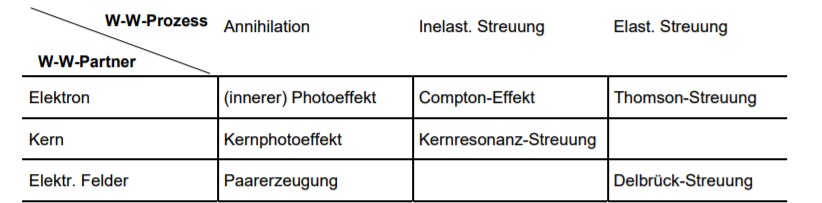
\includegraphics[height=4cm]{wechselwirkung.PNG}
  \caption{Verschiedene Effekte durch Wechselwirkungen von $\gamma$-Quanten. \cite{sample}}
  \label{fig:Linienspektrum}
\end{figure}

Die wichtigsten Effekte sind hierbei der Photoeffekt, der Compton-Effekt und die Paarbildung. Bei dem Photoeffekt wechselwirkt das
$\gamma$-Quant mit einem Hüllenelektron. Das $\gamma$-Quant wird vernichtet und das Elektron erhält dessen kinetische Energie.
Das Elektron wird aus seiner Schale gelöst wenn die Energie des $\gamma$-Quants größer ist als die Bindungsenergie des Elektrons.
Bei dem Compton-Effekt stößt das $\gamma$-Quant lediglich ein Elektron an und gibt einen Teil seiner Energie ab. Durch den Stoß
verändert sich die Bahn beider Teilchen. Durch diesen Effekt nimmt die Intensität eines $\gamma$-Strahls ab. Der
Wirkungsquerschnitt der Compton-Streuung ist definiert durch:
\begin{align}
  \sigma_{com} = 2 \pi r_e^2 \left(\frac{1+\epsilon}{\epsilon^2} \left[\frac{2(1+\epsilon)}{1+2\epsilon}-\frac{1}{\epsilon} ln(1+2\epsilon) \right]
                + \frac{1}{2\epsilon} ln(1+2\epsilon) - \frac{1+3\epsilon}{(1+2\epsilon)^2} \right)
\end{align}

Hierbei ist $\epsilon = E_{\gamma}/(m_0 c^2)$ das Verhältnis der Quantenenergie $E_{\gamma}$ zur Ruheenergie des Elektrons und
$r_e = \frac{e_0^2}{4 \pi \epsilon_0 m_0 c^2} = 2,82 \cdot 10^{-15}$m mit der Elektronenladung $e_0$ und der
Influenzkonstante $\epsilon_0$, der klassische Elektronenradius.

Für den Absorptionskoeffizient gilt:
\begin{align}
  \mu_{com} =\frac{z N_L}{M} \sigma_{com}
\end{align}

Die Paarbildung tritt auf, wenn die Energie des $\gamma$-Quants größer als die doppelte Ruhemasse des Elektrons ist. Dann
wird das $\gamma$-Quant unter der Bildung eines Elektrons und eines Positrons annihiliert.

Die drei genannten Effekte treten bei dem Durchgang eines $\gamma$-Strahls durch eine Materieschicht auf. Dementsprechend ist
der Absorptionskoeffizient kompliziert. In Abbildung 2 ist die Energieabhängigkeit des Absorptionskoeffizienten für Germanium zusehen.

\begin{figure}[H]
  \centering
  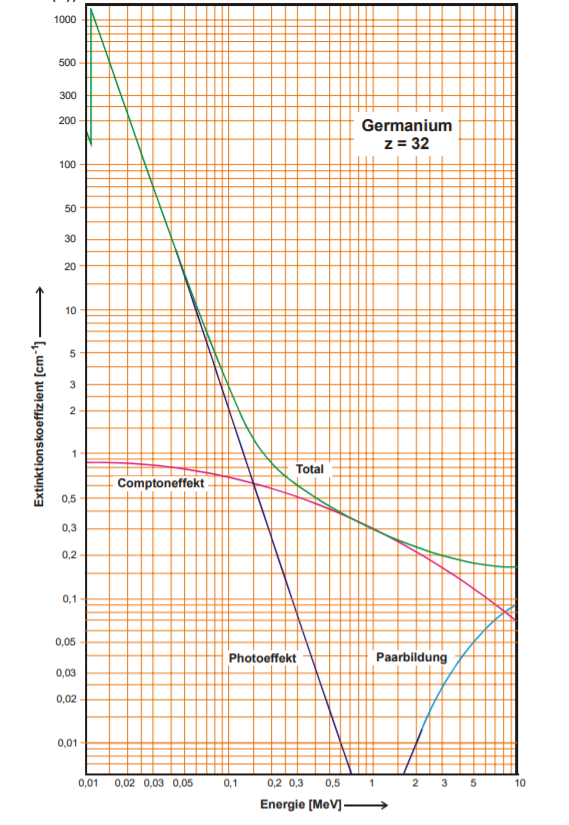
\includegraphics[height=12cm]{absorptionskoeffizient.PNG}
  \caption{Absorptionskoeffizent von Germanium in Abhängigkeit von der Energie \cite{sample}}
  \label{fig:Linienspektrum}
\end{figure}

Der Photoeffekt ist dabei für kleine Energien, der Compton-Effekt für mittlere Energien und die Paarbildung für
große Energien des $\gamma$-Quants von entscheidender Bedeutung.


\subsection{Beta-Strahlung}

Die $\beta$-Strahlung entsteht bei dem Zerfall von Atomkernen. Bei dem $\beta^{-}$-Zerfall zerfällt ein Neutron in ein Proton, ein Elektron
und ein Antineutrino, wobei das Elektron dabei als $\beta$-Teilchen bezeichnet wird. Der $\beta^{+}$-Zerfall beschreibt wie ein Proton in ein
Neutron, ein Positron und ein Neutrino zerfällt.
Die Energie verteilt sich dabei beliebig
auf das Elektron/Positron und das Neutrino/Antineutrino.
Die $\beta$-Teilchen erleiden beim Durchgang durch Materie wesentlich mehr Wechselwirkungen als bei der $\gamma$-Strahlung. Es werden
im wesentlichen 3 Prozessen voneinder unterschieden. Bei der elastischen Streuung werden die $\beta$-Teilchen von dem
Coulomb-Feld der Atomkerne abgelenkt, wodurch die $\beta$-Teilchen eine starke Ablenkung und auch geringe Energieverluste erfahren.
Bei der inelastischen Streuung werden die $\beta$-Teilchen von dem Coulomb-Feld der Atomkerne beschleunigt. Dadurch senden sie
Energie in Form von elektromagnetischer Strahlung ab, wodurch sie abgebremst werden.
Durch inelastische Streuung an den Elektronen des Absorbermaterials verlieren die $\beta$-Teilchen nur einen Bruchteil
ihrer Energie. Da diese Stöße jedoch sehr häufig Auftreten können und diese Wahrscheinlichkeit proportional zur Zahl der
Elektronen pro Volumeneinheit ist, können $\beta$-Teilchen durch diesen Prozess ihre gesamte Energie verlieren.

Für $\beta$-Teilchen aus natürlichen Quellen gilt bei nicht allzu großen Absorberschichtdicken näherungsweise Gleichung (2). Für
Schichtdicken in der Nähe der maximalen Reichweite $R_{max}$ der Teilchen weicht das Gesetzt deutlich ab. Oberhalb von dieser
Reichweite wird dann nur noch die Bremsstrahlung der $\beta$-Strahlung gemessen. In Abbildung 3 ist dies dargestellt.

\begin{figure}[H]
  \centering
  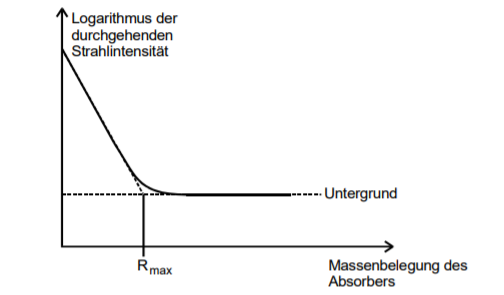
\includegraphics[height=8cm]{absorptionskurve.PNG}
  \caption{Absorptionskurve eines natürlichen Beta-Strahlers \cite{sample}}
  \label{fig:Linienspektrum}
\end{figure}

Die Massenbelegung $R$ hängt dabei von der Schichdicke ab:
\begin{align}
  R =\rho D
\end{align}

Da $R_{max}$ fast ausschließlich durch die energiereichsten Elektronen bestimmt ist, kann daraus die Größe $E_{max}$ berechnet werden.
Zwischen diesen beiden Größen gilt die Beziehung:
\begin{align}
  E_{max} = 1,92 \sqrt{R_{max}^2 + 0,22 R_{max}}
\end{align}
